\Level 0 {Introduction}

The `NP' stands for `nondeterministic polynomial time', which stands
for the fact that a solution can be checked (not: found) in polynomial
time.  This class of algorithms is informally characterized by the
fact there is polymomial time for checking their solution.
However, it is also true
that there is no polynomial algorithm known for solving them.

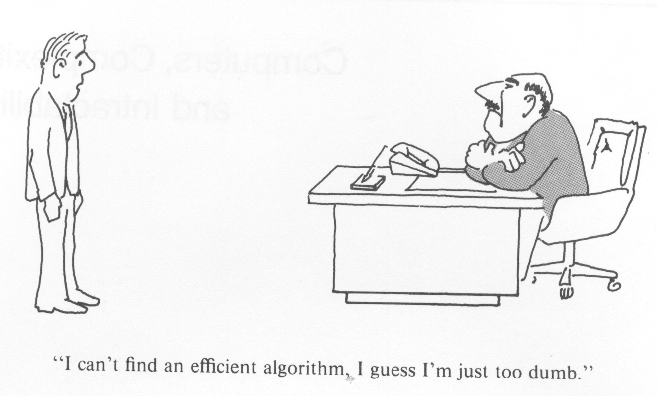
\includegraphics{np-dumb}

The fact that there is no efficient algorithms \emph{known} would not
be bad if it could be proved that no efficient algorithm
\emph{exists}.

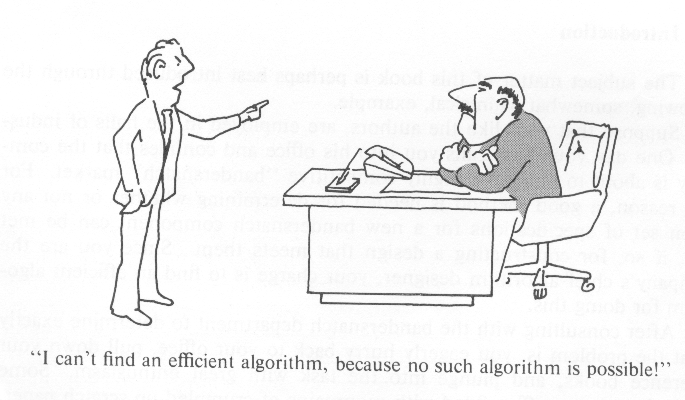
\includegraphics{np-prove}

However,
also there exists no non-polynomial lower bound on the solution
time. Thus, the question whether they can be solved in polynomial time
is still open. 
Since methods in this class can all be translated into
each other, having a solution method for one implies that methods
exist for all of them. This also means that none of the problems in
this class have been solved so far.

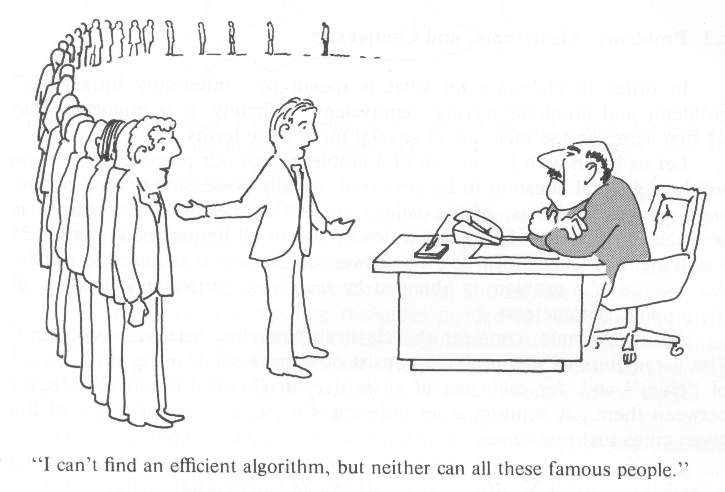
\includegraphics{np-famous}


\Level 0 {Basics}

\Level 1 {Optimization versus decision problems}

Many problems that are said to be NP-complete are optimization
problems. For instance, in the traveling salesman problem the shortest
route through a set of cities is asked. However, it is more convenient
to look at decision problems, that is, problems that have a yes or no
answer for each input.

It is not hard to transform an optimization problem into a decision
problem. Rather than asking for an optimal solution, we determine a
bound~$B$, and ask whether there is a solution that is within that
bound.
\begin{594exercise}
Finish this argument. Show that, if we can solve the optimization
problem, we can solve the decision problem. 
Now, supposing we can solve the decision problem, how
does that give a solution of the optimization problem? Assume that the
outcome of the optimization problem is an integer quantity. Do you
have to make other assumptions; discuss? What is
the complexity of the one solution method given a certain complexity
for the other?
\end{594exercise}
\begin{answer}
If the decision problem can be solved, the optimization problem can be
solved by asking about various values of the bound. This means the
decision problem will be solved a logarithmic number of times.
This only works if the bound takes on integer values; for rational or
irrational values bisection search will not terminate.

A second assumption is that lower and upper bounds are given. This is 
a reasonable assumption in many problems; for instance, in the
traveling salesman problem a linear time algorithm gives the sum of
all distances between cities, which is an upper bound. The lower bound
is zero.
\end{answer}

\Level 1 {Language of a problem}

For each optimization or decision problem we can defined `instances',
which are ways of setting all the free variables of the problem. Since
these variables are in sets of types that depend on the problem, we
can not be more precise here. A~problem can then be phrased as a
question over this set of instances: which instances optimize the cost
function, or which give a yes answer. That last set we will
denote~$Y_\Pi$.

Again depending on the problem, we can encode instances of a
problem. For instance, in the traveling salesman problem, an instance
would be encoded as the ordered list of cities to pass through.

With this, we can define the language of a problem:
\[ L[\Pi,e]=\{ \hbox{the instances in $Y_\Pi$ encoded under $e$} \} \]

\Level 1 {Turing machines}

A Turing machine, given some input, can halt with the yes state~$q_Y$,
the no state~$q_N$, or can never halt. We say that a string is
accepted if it leads the Turing machine to halt with~$q_Y$. The
language~$L_M$ of a Turing machine~$M$ is the set of strings that are accepted.

A deterministic Turing machine (DTM)~$M$ is said to solve a problem~$\Pi$
(under some encoding~$e$), or equivalently to recognize~$L[\Pi,e]$, if
\begin{itemize}
\item it halts for all strings over its input alphabet, and
\item its language $L_M$ is $L[\Pi,e]$.
\end{itemize}
Note that `solving a problem' here actually means `recognizing a
solution of the problem'. This DTM is a solution checker, not a
solution generator.

As an example, consider the recast  the traveling salesman problem
`does a route, shorter than~$B$, exist?'. The set of purported
solutions are then lists of cities, and the DTM gives for each list a
verdict `yes, this route is shorter than~$B$' or `no, this route is
not shorter than~$B$'.

\Level 0 {Complexity classes}

\Level 1 {Class P}

This allows us to define class~$P$:
\[ P=\{L:\hbox{there is DTM that recognizes $L$ in polynomial time}\} \]
and with this
\begin{eqnarray*}
 \Pi\in P&\equiv& L[\Pi,e]\in P\quad\hbox{for some encoding $e$}\\
        &\equiv&\hbox{there is a polynomial time DTM
                 that recognizes $L[\Pi,e]$}
\end{eqnarray*}
What this means is that for problems in~$P$ there is a polynomial time
Turing machine that recognizes strings in~$Y_\Pi$ as valid, and that
on strings not in~$Y_\Pi$ it both halts, and gives a negative verdict.

\Level 1 {Class NP}

Solving the traveling salesman problem may be hard, but if we have a
network and some bound, and 
someone gives us an itinerary with the claim that it satisfies that
bound, we can check this with a~DTM in polynomial time. We can now
build a non-deterministic Turing machine (NDTM) which `solves' such
problems:
given a decision problem it `guesses' some
purported solution, and then checks (with a DTM) whether that solves
the decision problem.
The guessed solution is called a `certificate'.

Clearly, only if the decision problem has an answer of~`true' can the
NDTM guess a solution, so the~$Y_\Pi$ of this problem is precisely the
set of decision problem instances with a yes answer.

For instance, for the traveling salesman problem, the instances
in~$Y_\Pi$ are a combination of a cities network plus a feasible bound
on the travel time. The non-deterministic Turing machine would then
guess an itinerary, and it can be checked in polynomial time that that
is indeed a valid route, and that is satisfies the bound.

We can write this whole story compactly: a problem~$\Pi$ is in~NP if
there is a polynomial time function~$A(\cdot,\cdot)$ such that
\[ w\in Y_\Pi \Leftrightarrow \exists_C:A(w,C)=\mathrm{true} \]
and $C$ itself can be polynomially generated.

The final condition on the generation of the certificate is needed for
a total polynomial runtime, but in practice it is not much of a
limitation. For instance, in the traveling salesman problem, a list of
cities can be guessed in linear time.

\begin{594exercise}
Prove that NP is closed under union and intersection. What difficulty
is there in showing that it is closed under complement taking?
\end{594exercise}

\Level 1 {Examples}

As was indicated above, while finding a solution to a problem is often
hard, checking that something is a solution is often fairly simply and
doable in polynomial time. A~nontrivial example of a polynomial time
problem is checking whether a number is prime. This question was only
settled in 2002. Before that there were polynomial time probabilistic
testers, which would test a number and return a verdict with high
reliability, or with a high probability of polynomial running time.
\begin{594exercise}
Why is the following algorithm not a linear time solution to the
\textsc{Prime} problem?
\begin{tabbing}
for \=$i=0\ldots\sqrt n$:\\
\>if \=$\mod(n,i)\equiv0$\\
\>\>return true
\end{tabbing}
\end{594exercise}
\begin{answer}
The modulo operation is not an $O(1)$ operation. For
$n\rightarrow\infty$, you have to take the length of the number into
account.
\end{answer}

Other algorithms have provably an exponential running time. Examples
here are finding the best move in chess, or checking statements in
Pressburger arithmetic.

It is possible to find levels in between polynomial and
exponential. The problem of factoring an integer (note that this is
more powerful than primality testing) has a runtime of
$O(\exp((n\cdot 64/9)^{1/3})(\log n)^{2/3})$. Interestingly, on a quantum
computer, a polymial algorithm is known; see
\url{http://en.wikipedia.org/wiki/Shors_algorithm}.

In the next section we will go further into the middle ground, of
algorithms for which no polymomial time algorithm is known, but for
which no exponential bound is known either.

\Level 0 {NP-completeness}

\Level 1 {Transformations}

Often it is possible to transform one problem into another. This has
the advantage that, if you prove that one problem is in a certain
class, the other one is also in that class. Of course this depends on
the nature of the transformation.

We will here consider `polynomial transformations'. Let $L_1$~and~$L_2$
be the languages of two problems over alphabets
$\sum_1^*$~and~$\sum_2^*$ respectively, then $f$~is a polymomial
transformation of problem~1 into problem~2 if
\begin{itemize}
\item There is a DTM that computes~$f(x)$ in time~$T_f(x)\leq p_f(|x|)$ for
  some polynomial~$p_f$, and
\item For all $x\in\sum_1^*$, $x\in L_1$ iff $f(x_1)\in L_2$.
\end{itemize}
The transformation does not have to be a one-to-one mapping, so it is
sometimes explicitly terms a `many-to-one polynomial transformation'.

\begin{lemma}
Suppose $f$ is a polynomial transformation from $L_1$~to~$L_2$,
then \[ L_2\in P\Rightarrow L_1\in P \]
\end{lemma}
Proof: assume that $M_2:L_2\rightarrow\{0,1\}$ is a DTM that
recognizes~$L_2$, then $M_2\circ f$~is a DTM that recognizes~$L_1$,
and this composition still runs in polynomial time~$T_{M_2\circ
  f}(x)\leq p_{T_2}(|p_f(|x|)|)$.

If $L_1$ transforms to $L_2$ (in polynomial time), we notate that as
$L_1\leq L_2$. This notation also suggests the idea that $L_1$ is
easier than~$L_2$.

It is easy to see that 
\[ L_1\leq L_2 \wedge L_2\leq L_3 \Rightarrow L_1\leq L_3, \]
that is, the `transforms into' relation is transitive.

\Level 1 {NP-complete}

A language~$L$ is said to be NP-complete if
\begin{itemize}
\item $L\in NP$, and
\item for all $L'\in NP$: $\L'\leq L$
\end{itemize}

(Languages that satisfy the second clause but not the first are called
`\index{NP-hard}NP-hard'. One example is the halting problem, which is
known not to be decidable. In other words, the DTM that should
recogize the language does not always halt with yes or no.)

Informally, the class NP-complete is that of the problems where a
solution can be verified quickly (meaning, in polynomial time). On the
other hand, P~is the class of problems where the solution can be
\emph{computed} quickly. The question whether these classes are
disjoint is open. In fact, you can win a million dollars by settling
it one way or another.

\begin{lemma}
If $L_1,L_2\in NP$, $L_1$ is NP-complete, and $L_1\leq L_2$, then
$L_2$ is NP-complete.
\end{lemma}
Proof: the only thing we need to check is that every $L'\leq L_2$ for
all~$L_2\in\nobreak NP$. Since $L_1$ is NP-complete, $L'\leq L_1$. Now
use the transitivity of the transform relation.

\Level 1 {Proving NP-completeness}

Above we saw that, given one NP-complete problem, others can easily be
proved NP-complete by constructing a mapping between the one problem
and the other. This raises a bootstrapping question.

Stephen Cook was the first to prove the NP-completeness of any problem
(1971), in his case the satisfiability problem. This is the problem
of, given boolean variables $x_1\ldots x_n$ and a logical formula
$F(x_1,\ldots,x_n)$, deciding whether there is a way of specifying the
variables such that the result is true.

Examples: the formula $x_1\vee\neq x_1$ is always true; $x_1\wedge\neq
x_1$ is always false, and $x_1\wedge \neq x_2$ is only true for the
pair~$(x_1=T,x_2=F)$. For the first and third examples, there are
values of $x_1,x_2$ for which the formula is true, so these are
satisfiable. The second example is not satisfiable.

\begin{comment}
There are several normal forms of this problem. The one used here is
the conjunction (by~AND) of clauses of the form $u_i\vee v_i$, where
$u_i,v_i$ are $x_j$ or~$\neq x_j$ for some values of~$j$.
\end{comment}

The Boolean satisfiability problem is in NP because a
non-deterministic Turing machine can guess an assignment of truth
values to the variables, determine the value of the expression under
that assignment, and accept if the assignment makes the entire
expression true.

Now, to prove that the satisfiability problem is NP-complete, it remains
to show that any language~$L\in NP$ can polynomially be transformed into
it. This is done by assuming a NDPT Turing machine for~$L$, and
transforming it into a logical formula, so that there is a
correspondence between successful computation in the NDTM, and a
satisfied logical formula.

Let the Turing machine be
\[ M = \langle Q, s, \Sigma, F, \delta\rangle
\]
where
\begin{description}
\item[$Q$] is the set of states, and $s\in Q$ the initial
       state,
\item[$\Sigma$] the alphabet of
     tape symbols,
\item[$F\subset Q$] the set of accepting states, and
\item[$\delta\subset Q\times\Sigma\times Q\times\Sigma\times\{-1,+1\}$] the
  set of transitions,
\end{description}
and that $M$ accepts or rejects an instance of the problem in time
$p(n)$ where $n$~is the size of the instance and $p(\cdot)$ is a
polynomial function.

We describe for each instance $I$ a Boolean expression which is
satisfiable if and only if the machine~$M$ accepts~$I$.

The Boolean expression uses the variables set out in the following
table, where $q\in Q$, $-p(n)\leq i\leq p(n)$, $j\in\Sigma$,
and~$0\leq k\leq p(n)$:

\begin{tabular}{|lp{2in}l|}
\hline
Variables&
Intended interpretation&
How many\\
\hline
$T_{ijk}$&
True iff tape cell $i$ contains symbol~$j$ at step~$k$ of the computation&
$O(p(n)^2)$\\
$H_{ik}$&
True iff the $M$'s read/write head is at tape cell~$i$ at step~$k$ of the computation.&
$O(p(n)^2)$\\
$Q_{qk}$&
True iff~$M$ is in state~$q$ at step~$k$ of the computation.&
$O(p(n))$\\
\hline
\end{tabular}


Define the Boolean expression~$B$ to be the conjunction of 
the clauses in table~\ref{table:cook}, for all 
$-p(n) \leq i\leq p(n)$, $j\in\Sigma$, and~$0\leq k\leq p(n)$.

\begin{table}[ht]
\begin{tabular}{|p{1in}p{1.6in}p{1.5in}p{.7in}|}
\hline
For all:&
Add the clauses&
Interpretation&
How many clauses?\\
\hline
\multicolumn{4}{|l|}{\textit{initial conditions}}\\
\hline
Tape cell~$i$ of the input~$I$ contains symbol~$j$.&
$T_{ij0}$&
Initial contents of the tape.&
$O(p(n))$
\\
&
$Q_{s0}$&
Initial  state of~$M$&
$O(1)$
\\
&
$H_{00}$&
Initial position of read/write head.&
$O(1)$
\\
\hline
\multicolumn{4}{|l|}{\textit{physical constraints}}\\
\hline
symbols $j \not=j'$&
$T_{ijk} \rightarrow \neg T_{ij'k}$&
One symbol per tape cell.&
$O(p(n)^2)$
\\
states $q \not=q'$&
$Q_{qk} \rightarrow  \neg  Q_{q'k}$&
Only one state at a time.&
$O(p(n))$
\\
cells $i \not=i'$&
$H_{ik} \rightarrow  \neg  H_{i'k}$&
Only one head position at a time.&
$O(p(n))$
\\
\hline
\multicolumn{4}{|l|}{\textit{Turing machine basics}}\\
\hline
$i,j,k$&
$T_{ijk} =T_{ij(k+1)} \vee H_{ik}$&
Tape remains unchanged unless written.&
$O(p(n)^2)$
\\
$f\in F$&
The disjunction of the clauses $Q_{f,p(n)}$&
Must finish in an accepting state.&
$O(1)$
\\
\hline
\multicolumn{4}{|l|}{\textit{transition table}}\\
\hline
$(q, \sigma ,q', \sigma', d) \in\delta$&
The disjunction of the clauses\newline
$(H_{ik} \wedge  Q_{qk} \wedge T_{i\sigma k})
\rightarrow  (H_{(i+d)(k+1)} \wedge Q_{q'(k+1)} \wedge T_{i\sigma' (k+1)})$&
Possible transitions at computation step~$k$ when head is at position~$i$.&
$O(p(n)^2)$
\\
\hline
\end{tabular}
\caption{Translation table from a NDPT Turing machine to a logic
  formula}
\label{tab:cook}
\end{table}

This table describes how to construct a logical formula in the
variables $T_{ijk},H_{ik},Q_{qk}$ (describing tape contents, head
positions, and states, respectively) that corresponds to the Turing
machine.
If there is an accepting computation for~$M$ on input~$I$, then~$B$ is
satisfiable, by assigning $T_{ijk}$, $H_{ik}$ and~$Q_{ik}$ their
intended interpretations. On the other hand, if~$B$ is satisfiable,
then there is an accepting computation for~$M$ on input~$I$ that
follows the steps indicated by the assignments to the variables.

How large is~$B$? There are $O(p(n)^2)$ Boolean variables, each of
which may be encoded in space $O(\log p(n))$. The number of clauses is
$O(p(n)^2)$. So the size of~$B$ is $O((\log p(n))p(n)^2)$. This is
polynomial in $n$, the size of the input, so the transformation is
certainly a polynomial-time reduction, as required.

